\documentclass{scrreprt}

\usepackage{aligned-overset}
\usepackage{amsmath}
\usepackage{amsthm}
\usepackage{amssymb}
\usepackage{bm}
\usepackage[inline,shortlabels]{enumitem}
\usepackage{hyperref}
\usepackage[utf8]{inputenc}
\usepackage{multicol}
\usepackage{mathtools}
\usepackage{pdflscape}
\usepackage{physics}
\usepackage{tabularx}
\usepackage[table]{xcolor}
\usepackage{titling}
\usepackage{fancyhdr}
\usepackage{xfrac}
\usepackage{pgfplots}

\pgfplotsset{compat = newest}
\usepgfplotslibrary{fillbetween}
\usetikzlibrary{calc}


\author{Karsten Lehmann}
\date{SoSe 2025}
\title{Übungsblatt 05\\INF-B-120, Mathematische Methoden für Informatiker}

\setlength{\parindent}{0pt}

\setlength{\headheight}{26pt}
\pagestyle{fancy}
\fancyhf{}
\lhead{\thetitle}
\rhead{\theauthor}
\lfoot{\thedate}
\rfoot{Seite \thepage}

\begin{document}
\paragraph{Ü 5.1} Verwenden Sie den Zwischenwertsatz um zu zeigen, dass
\begin{enumerate}[(a)]
\item die Funktion $f\qty\big(x) = e^x + x$ eine Nullstelle besitzt.

  \subparagraph{Lsg.} Es ist $f\qty\big(0) = e^0 + 0 = 1$ und
  $f\qty\big(-1) = e^{-1} - 1 \approx \frac{1}{2.718} - 1 < 0$.

  Nun folgt aus dem Zwischenwertsatz, dass die Funktion $f$ auf dem
  Intervall $\qty\big[-1, 0]$ eine Nullstelle besitzt.

  \begin{tikzpicture}[scale=.9]
    \begin{axis}[
      axis x line=center,
      axis y line=center,
      grid=both,
      samples=200,
      xmin=-2.5,
      xmax=2.5,
      xtick distance=1,
      ymin=-2.5,
      ymax=2.5,
      ytick distance=1,
    ]
      \addplot[domain=-2:2, smooth] { (e^x + x) };
    \end{axis}
  \end{tikzpicture}

\item die Funktionen $f\qty\big(x) = e^x - x$ und $g\qty\big(x) = 2 - x^2$
  mindestens zwei Schnittpunkte haben.

  \subparagraph{Lsg.} Sei
  \begin{flalign*}
    h\qty\big(x) &= f\qty\big(x) - g\qty\big(x) \\
                 &= e^x - x - \qty\big(2 - x^2) \\
                 &= e^x - x - 2 + x^2
  \end{flalign*}
  Nun ist $h\qty\big(0) = -1$ und $h\qty\big(1) = e - 2 < 0$
  sowie $h\qty\big(-1) = e$.

  Es folgt aus dem Zwischenwertsatz, dass $h\qty\big(x)$ auf den Intervallen
  $\qty\big[-1, 0]$ und $\qty\big[0, 1]$ jeweils (mindestens) eine Nullstelle
  und somit $f$ und $g$ Schnittpunkte besitzen.

  \begin{tikzpicture}[scale=.9]
    \begin{axis}[
      axis x line=center,
      axis y line=center,
      grid=both,
      samples=200,
      xmin=-2.5,
      xmax=2.5,
      xtick distance=1,
      ymin=-2.5,
      ymax=2.5,
      ytick distance=1,
    ]
      \addplot[domain=-2:2, smooth] { (2 - x * x) };
      \addplot[domain=-2:2, smooth] { (e^x - x) };
    \end{axis}
  \end{tikzpicture}

\end{enumerate}

\paragraph{Ü 5.2} Gegeben sind die beiden Funktionen
\[
  f \colon \qty\big(-1, \infty) \to \mathbb{R},
  f\qty\big(x) \coloneqq \ln\qty\big(x + 1)
  \text{ und }
  g \colon \mathbb{R} \to \mathbb{R},
  g\qty\big(x) \coloneqq x - x^2
\]
Bestimmen Sie alle $x \in \mathbb{R}$ für die $f$ und $g$ an der Stelle $x$ eine
gemeinsame Tangente besitzen.

\subparagraph{Lsg.} Die beiden Funktionen besitzen an der Stelle $x$ eine
gemeinsame Tangente, falls $f\qty\big(x) = g\qty\big(x)$ und
$f'\qty\big(x) = g'\qty\big(x)$.

Nun ist $f'\qty\big(x) = \frac{1}{x + 1}$ und $g'\qty\big(x) = 1 - 2x$.
Durch gleichsetzen der Ableitungen erhält man
\begin{flalign*}
  \frac{1}{x + 1} &= 1 - 2x && {\Big |} \cdot \qty\big(x + 1) \\
  1 &= \qty\big(1 - 2x)\qty\big(x + 1) \\
                  &= x + 1 -2x^2 - 2x && {\Big |} - 1 \\
  0 &= -2x^2 - x && {\Big |} \cdot \qty\big(-1) \\
                  &= x\qty\big(2x + 1)
\end{flalign*}
$\Rightarrow x_1 = 0$ und $x_2 = -\frac{1}{2}$.

Nun ist $f\qty\big(0) = \ln\qty\big(1) = 0 = g\qty\big(0)$, somit besitzen die
beiden Funktion an der Stelle $x = 0$ tatsächlich eine gemeinsame Tangente.
Allerdings ist
$f\qty(-\frac{1}{2}) = \ln\qty(\frac{1}{2}) \ne -\frac{3}{4} = g\qty(-\frac{1}{2})$
und somit $x = 0$ auch die einzige gemeinsame Tangente.

\paragraph{Ü 5.3} Bestimmen Sie für die folgenden reellen Funktionen $f$ jeweils
\begin{itemize}
\item die Ableitung $f'$
\item alle Stellen $x$, an denen die Funktion Extrema (Minima und Maxima) besitzt
\item alle größtmöglichen Intervalle, in denen die Funktion streng monoton ist.
\end{itemize}

\begin{enumerate}[(a)]
\item $f\qty\big(x) \coloneqq \frac{1}{x^2 - 6x + 10}$

  \subparagraph{Lsg.} Seien $g\qty\big(x) = 1$ und $h\qty\big(x) = x^2 - 6x + 10$.
  Dann ist nach der Quotientenregel
  \[
    f'\qty\big(x)
    = \frac{g'\qty\big(x) \cdot h\qty\big(x) - g\qty\big(x) \cdot h'\qty\big(x)}{\qty(h\qty\big(x))^2}
    = \frac{6 - 2x}{\qty\big(x^2 - 6x + 10)^2}
  \]
  Nun ist $0 = f'\qty\big(x) \iff x = 3$.
  Durch Betrachtung der Umgebung von $x = 3$ auf $f'$ fällt auf, dass
  $f'\qty\big(x) > 0$ für $x < 3$ und $f'\qty\big(x) < 0$ für $x > 3$.

  Es folgt, dass $f$ auf $\qty\big(-\infty, 3)$ streng monoton steigend und auf
  $\qty\big(3, \infty)$ streng monoton fallend ist.
  Damit hat $f$ bei $x = 3$ ein Maximum.

\newpage
\item $f\qty\big(x) \coloneqq x \cdot \qty(\ln\qty\big(x))^2$

  \subparagraph{Lsg.} Seien $a\qty\big(x) = x$, $b\qty\big(x) = x^2$ sowie
  $c\qty\big(x) = \ln\qty\big(x)$.
  Dann ist $f\qty\big(x) = a\qty\big(x) \cdot b\qty(c\qty\big(x))$.

  Somit ist nach der Kettenregel
  \[
    \qty(b \circ c)'\qty\big(x) = \frac{2\qty(\ln\qty\big(x))}{x}
  \]
  sowie nach der Produktregel
  \begin{flalign*}
    f'\qty\big(x)
    &= a'\qty\big(x) \cdot b\qty\big(c\qty\big(x)) + a\qty\big(x) \cdot \qty(b \circ )'\qty\big(x) \\
    &= \qty(\ln\qty\big(x))^2 + x \cdot \frac{2\qty(\ln\qty\big(x))}{x} \\
    &= \qty(\ln\qty\big(x))^2 + 2\ln\qty\big(x) = \ln\qty\big(x) \cdot (\ln\qty\big(x) + 2)
  \end{flalign*}
  Schließlich ist $f'\qty\big(x) = 0$ für $x_1 = 1$ und $x_2 = e^{-2}$.

  Nun ist $f\qty\big(x_1) = f\qty\big(0) = 0$.
  Betrachtet man die Umgebung von $x_1$ auf $f$ fällt auf, dass $f\qty\big(x) > 0$
  für $x \to x_1$.
  Somit besitzt $f$ ein Minimum an $x_1$.

  Analog ist $f\qty\big(x_2) = f\qty(e^{-2}) = e^{-2} \cdot \qty(\ln\qty(e^{-2}))^2 = \frac{4}{e^2}$.
  Nun könnte man entweder wieder die Umgebung von $x_2$ auf $f$ oder $f'$
  betrachten oder sogar die zweite Ableitung ermitteln.

  Oder man schließt von dem Minima $x_1$, genau zwei Nullstellen der ersten
  Ableitung und $\displaystyle \lim_{x \to 0+}f\qty\big(x) = 0$ direkt auf ein
  Maximum an $x_2$.

  Schließlich ist $f$ auf $\qty\big(0, e^{-2})$ streng monoton steigen,
  auf $\qty\big(e^{-2}, 1)$ streng monoton fallend und
  $\qty\big(1, \infty)$ wieder streng monoton steigend.

\newpage
\item $f\qty\big(x) \coloneqq \frac{x}{\sqrt{5 - x}}$

  \subparagraph{Lsg.} Seien $a\qty\big(x) = x$, $b\qty\big(x) = \sqrt{x}$ sowie
  $c\qty\big(x) = 5 - x$.
  Dann ist $f\qty\big(x) = \frac{a\qty\big(x)}{b\qty(c\qty\big(x))}$.

  Somit ist nach der Kettenregel
  \[
    \qty(b \circ c)'\qty\big(x) = \frac{1}{2} \cdot \qty\big(5 - x)^{-\frac{1}{2}}
    = \frac{1}{2\sqrt(5 - x)}
  \]
  sowie nach der Quotientenregel
  \begin{flalign*}
    f'\qty\big(x)
    &= \frac{a'\qty\big(x) \cdot b\qty(c\qty\big(x)) - a\qty\big(x) \cdot \qty(b \circ c)'\qty\big(x)}{\qty(b\qty\big(c\qty\big(x)))^2} \\
    &= \frac{\sqrt{5 - x} - \frac{x}{2\sqrt{5 - x}}}{5 - x} \\
    &= \frac{\frac{10 - 2x}{2\sqrt{5 - x}} - \frac{x}{2\sqrt{5 - x}}}{5 - x} \\
    &= \frac{\frac{10 - x}{2\sqrt{5 - x}}}{5 - x} \\
    &= \frac{10 - x}{2\sqrt{5 - x} \cdot \qty\big(5 - x)}
  \end{flalign*}
  Nun ist $x = 10$ keine Nullstelle von $f'$, da die Wurzel für negative Zahlen
  nicht definiert ist und $f$ somit nur auf $\qty\big(-\infty, 5)$ definiert ist.
  Es folgt $10 - x > 0$, $5 - x > 0$ und sowieso $2\sqrt{5 - x} > 0$.
  Damit ist $f$ im gesamten Definitionsbereich streng monoton steigend und
  besitzt keine Minima oder Maxima.
\end{enumerate}

\newpage
\paragraph{Ü 5.4} Wir betrachten die Funktion
$f \colon \qty\big(0, \pi) \to \qty\big(-1, 1)$
mit $f\qty\big(x) \coloneqq \cos\qty\big(x)$.

Verwenden Sie die Formel für die Ableitung der Umkehrfunktion, um die
Ableitung der Funktion $f^{-1}\qty\big(x) = \arccos\qty\big(x)$ zu berechnen.

(Dabei ist die Gleichung $\sin^2\qty\big(x) + \cos^2\qty\big(x) = 1$ hilfreich.)

\subparagraph{Lsg.} Betrachte zuerst
\begin{flalign*}
  \sin^2\qty\big(x) + \cos^2\qty\big(x) &= 1 && {\Big |} - \cos^2\qty\big(x) \\
  \sin^2\qty\big(x) &= 1 - \cos^2\qty\big(x) && {\Big |} \sqrt{\ldots} \\
  \sin\qty\big(x) &= \sqrt{1 - \cos^2\qty\big(x)} \quad \qty\big(\textbf{*})
\end{flalign*}
Sei nun  $x \in \qty\big(-1, 1)$ beliebig.
Dann ist
\begin{flalign*}
  f\qty(f^{-1}\qty\big(x)) = x &\iff \qty\Big(f\qty(f^{-1}\qty\big(x)))' = 1 \\
                               &\iff \qty\Big(\cos\qty(\arccos\qty\big(x)))' = 1 \\
  \overset{\text{Kettenregel}}&\iff -\sin\qty(\arccos\qty\big(x)) \cdot \qty(\arccos\qty\big(x))' = 1 \\
  \overset{f^{-1} \colon \qty\big(-1, 1) \to \qty\big(0, \pi), f^{-1}\qty\big(x) \ne 0}&\iff \qty(\arccos\qty\big(x))' = -\frac{1}{\sin\qty(\arccos\qty\big(x))} \\
  \overset{\qty\big(\textbf{*})}&\iff \qty(\arccos\qty\big(x))' = -\frac{1}{\sqrt{1 - \cos^2\qty(\arccos\qty\big(x))}} \\
  &\iff \qty(\arccos\qty\big(x))' = -\frac{1}{\sqrt{1 - x^2}}
\end{flalign*}

\end{document}
